%%
%% This is file `sample-sigconf.tex',
%% generated with the docstrip utility.
%%
%% The original source files were:
%%
%% samples.dtx  (with options: `sigconf')
%% 
%% IMPORTANT NOTICE:
%% 
%% For the copyright see the source file.
%% 
%% Any modified versions of this file must be renamed
%% with new filenames distinct from sample-sigconf.tex.
%% 
%% For distribution of the original source see the terms
%% for copying and modification in the file samples.dtx.
%% 
%% This generated file may be distributed as long as the
%% original source files, as listed above, are part of the
%% same distribution. (The sources need not necessarily be
%% in the same archive or directory.)
%%
%% The first command in your LaTeX source must be the \documentclass command.
\documentclass[sigplan]{acmart}

\usepackage{code}
\usepackage{graphicx}

%%
%% \BibTeX command to typeset BibTeX logo in the docs
\AtBeginDocument{%
  \providecommand\BibTeX{{%
    \normalfont B\kern-0.5em{\scshape i\kern-0.25em b}\kern-0.8em\TeX}}}

%%% The following is specific to Onward! '21 and the paper
%%% 'Let a Thousand Flowers Bloom: On the Uses of Diversity in Software Testing'
%%% by Alex Groce.
%%%
\setcopyright{acmcopyright}
\acmPrice{15.00}
\acmDOI{10.1145/3486607.3486772}
\acmYear{2021}
\copyrightyear{2021}
\acmSubmissionID{onward21essays-id2-p}
\acmISBN{978-1-4503-9110-8/21/10}
\acmConference[Onward! '21]{Proceedings of the 2021 ACM SIGPLAN International Symposium on New Ideas, New Paradigms, and Reflections on Programming and Software}{October 20--22, 2021}{Chicago, IL, USA}
\acmBooktitle{Proceedings of the 2021 ACM SIGPLAN International Symposium on New Ideas, New Paradigms, and Reflections on Programming and Software (Onward! '21), October 20--22, 2021, Chicago, IL, USA}


%%
%% Submission ID.
%% Use this when submitting an article to a sponsored event. You'll
%% receive a unique submission ID from the organizers
%% of the event, and this ID should be used as the parameter to this command.
%%\acmSubmissionID{123-A56-BU3}

%%
%% The majority of ACM publications use numbered citations and
%% references.  The command \citestyle{authoryear} switches to the
%% "author year" style.
%%
%% If you are preparing content for an event
%% sponsored by ACM SIGGRAPH, you must use the "author year" style of
%% citations and references.
%% Uncommenting
%% the next command will enable that style.
%%\citestyle{acmauthoryear}

%%
%% end of the preamble, start of the body of the document source.
\begin{document}

%%
%% The "title" command has an optional parameter,
%% allowing the author to define a "short title" to be used in page headers.
\title{Let a Thousand Flowers Bloom: on the Uses of Diversity in
  Software Testing}

%%
%% The "author" command and its associated commands are used to define
%% the authors and their affiliations.
%% Of note is the shared affiliation of the first two authors, and the
%% "authornote" and "authornotemark" commands
%% used to denote shared contribution to the research.
\author{Alex Groce}
\affiliation{\institution{Northern Arizona University}\country{United States}}


%%
%% By default, the full list of authors will be used in the page
%% headers. Often, this list is too long, and will overlap
%% other information printed in the page headers. This command allows
%% the author to define a more concise list
%% of authors' names for this purpose.
\renewcommand{\shortauthors}{Alex Groce}

%%
%% The abstract is a short summary of the work to be presented in the
%% article.
\begin{abstract}
Software testing is \emph{hard}, and a testing problem is composed of
many sub-problems with different, often conflicting, solutions.  Like many real-world problems, it
admits no single optimal solution, but requires dexterity, and the
opportunistic combination of many partial solutions.  Exploration and
experiment, even by practitioners, are important in real-world
critical testing efforts.  An important set of research results in the
field endorse and codify the value of \emph{diversity} in test generation.
However, our current approaches to evaluating research results
arguably cut against this fundamental reality: while effective testing
may need true diversity, combining many partial answers, the iron
logic of the research results section often imposes a
\emph{totalizing} vision where authors must at least pretend to
present a monolithic, unitary solution, a new ``king of the hill.''
\end{abstract}

\begin{CCSXML}
<ccs2012>
<concept>
<concept_id>10011007.10010940.10010992.10010998.10011001</concept_id>
<concept_desc>Software and its engineering~Dynamic analysis</concept_desc>
<concept_significance>500</concept_significance>
</concept>
<concept>
<concept_id>10011007.10011074.10011099.10011102.10011103</concept_id>
<concept_desc>Software and its engineering~Software testing and debugging</concept_desc>
<concept_significance>500</concept_significance>
</concept>
</ccs2012>
\end{CCSXML}

\ccsdesc[500]{Software and its engineering~Dynamic analysis}
\ccsdesc[500]{Software and its engineering~Software testing and debugging}

\keywords{software testing, test diversity, swarm testing, ensemble methods,
  test length, research evaluation methods}


\maketitle

\section{Introduction}

\begin{quote}
  ``Variety's the very spice of life,\\
  That gives it all its flavour.''
  \\ - William Cowper, ``The Task''
  \end{quote}

Discovering all the bugs in a software system is an extremely
difficult task.  It is so difficult, in fact, that in the real world
it is seldom really attempted, for most kinds of software.  However,
when software bugs can produce catastrophic consequences, as in the
case of safety-critical software, or produce catastrophic monetary or
institutional credibility
loss (e.g., a billion dollar Mars rover mission fails because of a bug
\cite{Spirit}), it is worth at least trying to find \emph{all} the bugs,
given our difficulty in estimating the probability that an
undiscovered bug will trigger in practice.

The difficulty in discovering bugs in software is not, alas, even of
a simple kind.  It is conceivable that, while ``truly thorough testing'' or
``complete verification'' would be \emph{costly} and \emph{require
  extensive human resources}, the methods for achieving these goals
would be widely known, and omitted out of simple cost-benefit
calculations.  Unfortunately, even given will-power and budget, we
generally don't know the best way to go about trying to find all the
bugs in a system.  Complete verification, for many real-world systems,
is often essentially impossible, and even if possible would rely on a
formal specification that might not represent important requirements.
And, in testing, we seldom know which approach to testing will work
best.  Even given a particular ``method,'' such as \emph{fuzzing}, it
turns out that the ability of experts to predict which approach(es)
will be most effective is limited.  Ask ten fuzzing researchers or
practitioners what the best fuzzer is, and you won't get ten answers;
but you certainly won't get just one answer, and you may well get more
than three different answers!

Moreover, even if everyone agreed on the best fuzzer, running just
that fuzzer would likely be a bad decision!  Different fuzzers are
best at discovering different bugs, for almost all software programs.
Any competitive fuzzer that is not strictly worse than another (e.g.,
the exact same fuzzer, but slower) is likely to have some bug(s) for
which it is better than the ``best'' fuzzer.

The need for multiple approaches is even more complex when we consider
that some bugs may be best detected by code review, some bugs may be
best detected by manually written unit or integration tests, some bugs
may be best detected by turning up the toleration for false positives
in static analysis, and being willing to wade through all the
resulting complaints, and so forth.  However, even if we limit the
topic to automated test generation methods, the fact remains.  There
are a very large number of possible approaches, and users serious
about finding bugs may easily miss important bugs if they only use one
of these methods, or even if they use a few of the best methods.  In
other words, this is a situation where the utility of \emph{diversity}
is extremely high.  Diversity, here, means employing a \emph{variety} of different
methods, where in some sense many of these methods may be \emph{worse}
(on average!) than others.

One way to understand the fundamental need for diversity in software
test generation is to think about the testing problem as an instance
of the coupon collector's problem \cite{FormalCoupon}.  The
generalized coupon
collector's problem \cite{coupon} is a probability problem in which
colored balls are drawn from an urn, with replacement.  In testing,
typically, there are many more balls than colors (distinct faults,
including the non-fault of a test that exposes no bugs); in fact,
under a particular test generation strategy, the distribution of bugs
often follows a severe power law, with some bugs extremely rare and
others very frequent \cite{Taming}\footnote{In fact, getting out of a
  bad distribution where the undetected bugs are very rare is one
  rationale for diversity in test generation; even a distribution
  where failing tests are very rare can be very useful if some
  previously rare bug is now made less impossible to find.}.
Collecting all the ``coupons'' in such a setting is difficult, \emph{even if
you can bias the selection of balls}, since many methods of bias will
only work for the balls whose chromatic properties you have already
observed, which might make it harder to find novel colors.

Testing is, therefore,
fundamentally, not best seen as an \emph{optimization} problem, at
least not a simple optimization problem, since
there is no single solution\footnote{Obviously, minimally, there is no single ``best
test'' and potentially there is no truly optimal strategy, when strategies do not
include mixed approaches.}.  We want to hit \emph{all} the bugs; moreover, since we have
no idea where the bugs are, we probably want to hit all of some set of
coverage targets, or synthetic bugs (as in mutation testing)
\cite{Discontents}.  Perhaps, in fact, coupon collection, while useful
as a tool for mathematical analysis, is the wrong analogy.  A better
way to think of software testing is as a \emph{scavenger hunt}, where
it might be a good idea to split up the team, since finding a teacup
with blue flowers and finding a Bunsen burner will probably involve
trips to very different locations.  Some trips may be fruitless
(perhaps the local tea-room has only green flowers, or even plain white
teacups), but cannot be omitted, without increasing the chance of
missing some items on the list.  Of course, in the case of bugs, the
matter is complicated by the fact that the list of items to be found
is not given to the team.

This essay could, at this point, turn to marshaling evidence that a
variety of approaches, even if some are ``inferior'' to others, is
needed for finding most bugs.  The research literature and practical
commentary includes substantial evidence for this fact.  Some of it
will be cited below; however, I think this isn't really very useful.
Few software testing researchers probably don't know that there is, to
particularize Brooks' general principle \cite{Brooks1987NoSB}, ``no silver bullet'' in test
generation.  Even fewer serious practitioners of software testing who
are any good at it will think there is such a thing.  However, many
seasoned testers may use only one method, or a handful of methods,
because of the problem of diversity.  If you are using one, known
pretty-good, method for automatically generating tests, the best
practice is likely pretty clear:  throw as many computing resources
into running this method as you can, and try to solve the hard problem
of triaging the resulting bugs and false positives you run into.  But
what if you want to use a diverse set of methods?  Learning to use one
method or tool is often time-consuming; learning to use every method
and tool sounds like a nightmare.  Two solutions offer themselves:
first, there are some ways to introduce diversity into testing even
with a single approach, that apply to many tools.  Second, there are
solutions that act as front-ends to diverse arrays of methods, saving
the bug-finder the effort of learning to ``talk'' to each approach in
its own unique language \cite{WODACommon}.

This essay will consider two aspects of this state of affairs.  First,
there is advice for the working bug-finder (developer, test engineer, systems
engineer, security auditor); what diversity-aware approaches are
available, to minimize the burden on the humble bug-finder, and make
it possible to act as if you are using one, best, method?  Second, and
perhaps in the long run 
more importantly, there is the problem that \emph{there is a serious
divergence between software testing research expectations and
publication barriers and the actual problems and solutions of software testing in a
diversity-critical world}.

\section{Digression: Diversity in General}

The idea that diversity is good is not novel, or specific to software
testing, of course.  The title of this essay is cobbled together from
famous phrases relating to the virtues of diversity \cite{chesterton,mao}.  Since, at least,
Montaigne \cite{montaigne}, Cervantes' \cite{cervantes} admonition to not ``put all your eggs in one
basket'', or perhaps the unknown Scotsman who said that it is good we all
don't like the same things, or there would be a powerful shortage of
oatmeal, diversity has been lauded, on occasion, in literature and
philosophy.  The idea of the American political system as using states
as the ``laboratory of democracy'' is essentially diversity-based, as
are arguments against too much central regulation by the European
Union.  Arguably, the same could be said for the city-states of the
ancient world (perhaps there is something to be said for both Athens
and Sparta, someone must have pointed out).  And, of course, diversity
is a widely embraced principle today: ACM has a council on Diversity
and Inclusion.

There are moral, ethical,
political, philosophical, utilitarian, and, especially,
aesthetic, arguments for preferring a multifarious, rather than
monolithic, world.  This essay is only concerned with the \emph{utilitarian}
approach to diversity exemplified by the folk saying about not putting
all your eggs in one basket.  If you only run one (very good!) fuzzer
and it happens to be bad at finding the most dangerous security
vulnerability in your code, you will be at least as unhappy as the young maid
who trips and pitches her one big basket of eggs on the ground in 17th
century Spain.  We don't care (inside this essay) if diversity is right, or
diversity is pretty, we just care that it is useful.

\section{Diversity in Practice}

In case anyone who actually goes about finding bugs in software is
reading this essay, let's start by looking at some existing ways of
making use of diversity.  The first two approaches described will
introduce ``meta-diversity'' --- diversity within a single tool or
method.  These approaches describe ways to make the behavior of a
single automated test generation method more diverse, with relatively
little effort.  They do not always apply to all methods, and, of
course, as the nature of the problem this essay faces suggests,
sometimes they don't work very well!  But they are worth trying, as
low-cost ways to add diversity when you can't, or don't want to, learn
a new method or tool.

The third approach described is fundamentally based on the uses of
diversity:  using \emph{ensemble} methods to allow a ``single'' tool
to (behind the scenes) apply many methods, with the explicit
rationale that diversity is useful in test generation.

\subsection{Test Length}

Most automated test generation tools have a notion of maximum length
of the tests generated.  For fuzzers, this will often be a number of
bytes; for API-call sequence generation, it will be the number of
calls in each test.  Most tools have default values for this
parameter, and few users probably change those values.  However, the
value length can have a huge impact on the testing, and the impact is
not as simple as there being an optimal value for the length
\cite{ASE08}; different bugs may ``want'' different lengths!

\begin{figure*}
  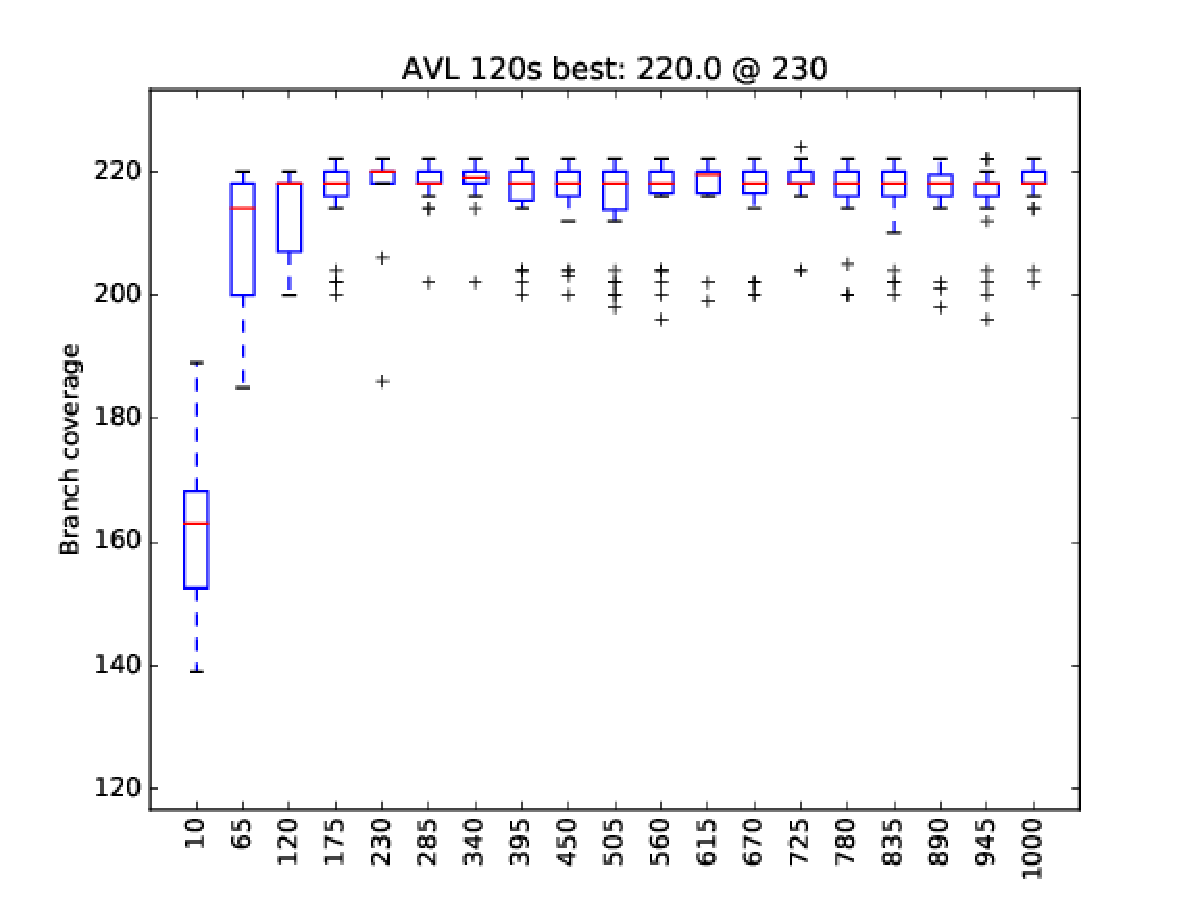
\includegraphics[width=0.9\columnwidth]{graphs/AVLrand120}
  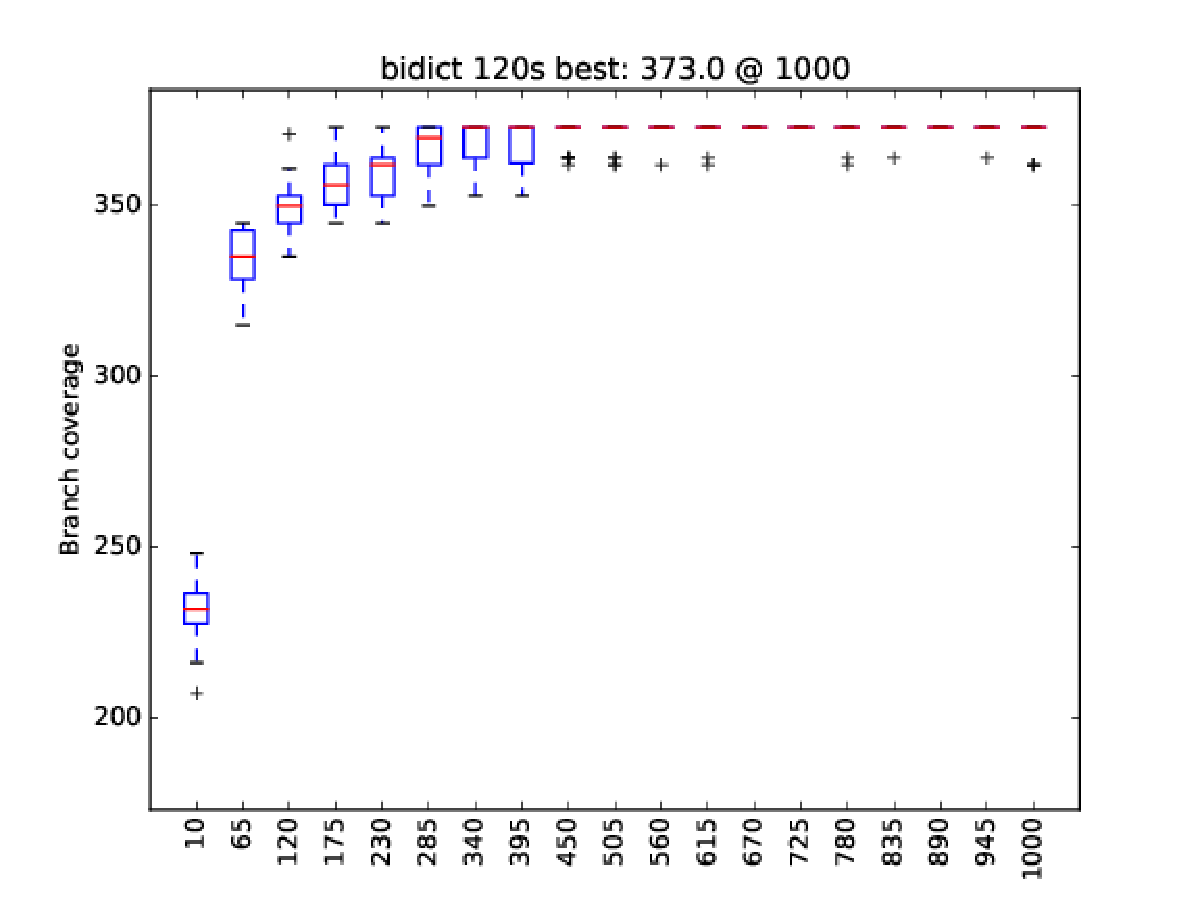
\includegraphics[width=0.9\columnwidth]{graphs/bidictrand120}
% 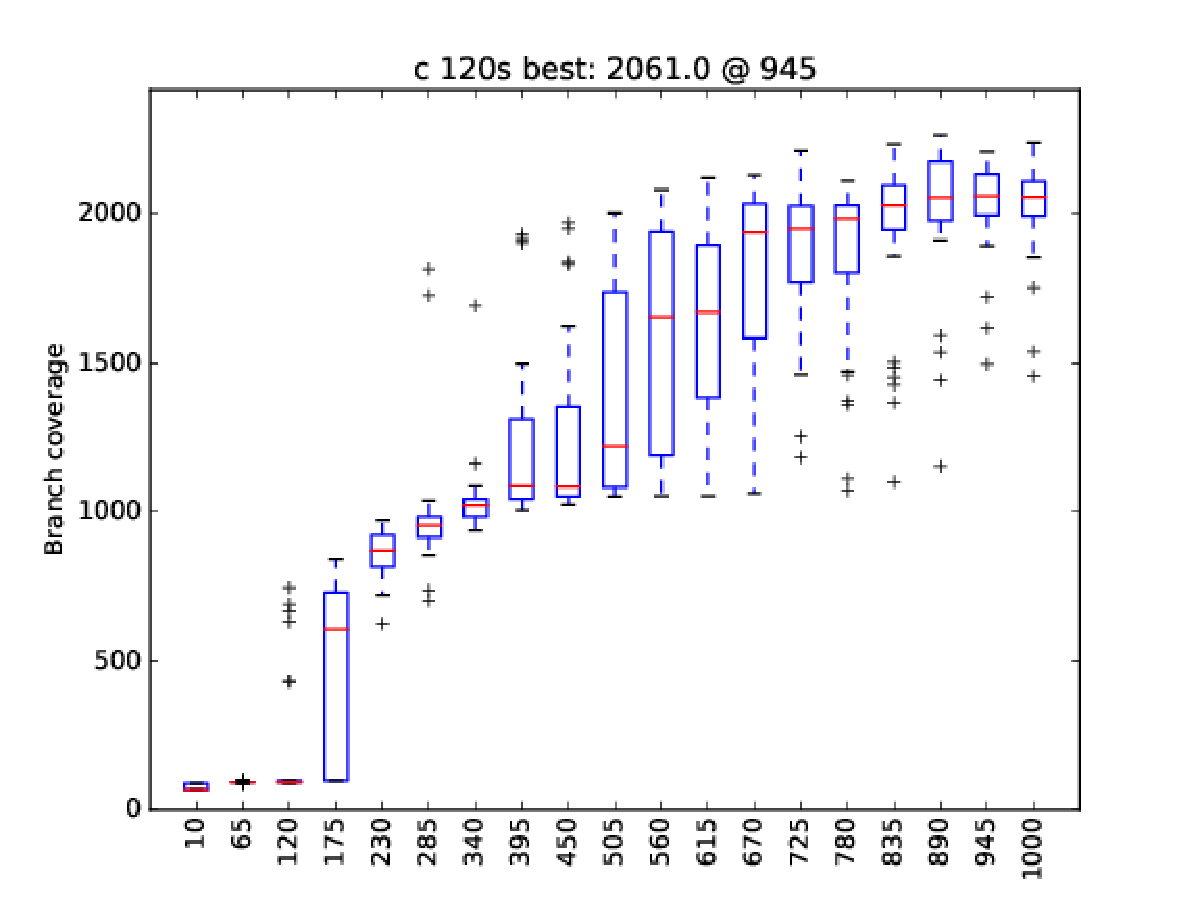
\includegraphics[width=0.9\columnwidth]{graphs/Crand120} 
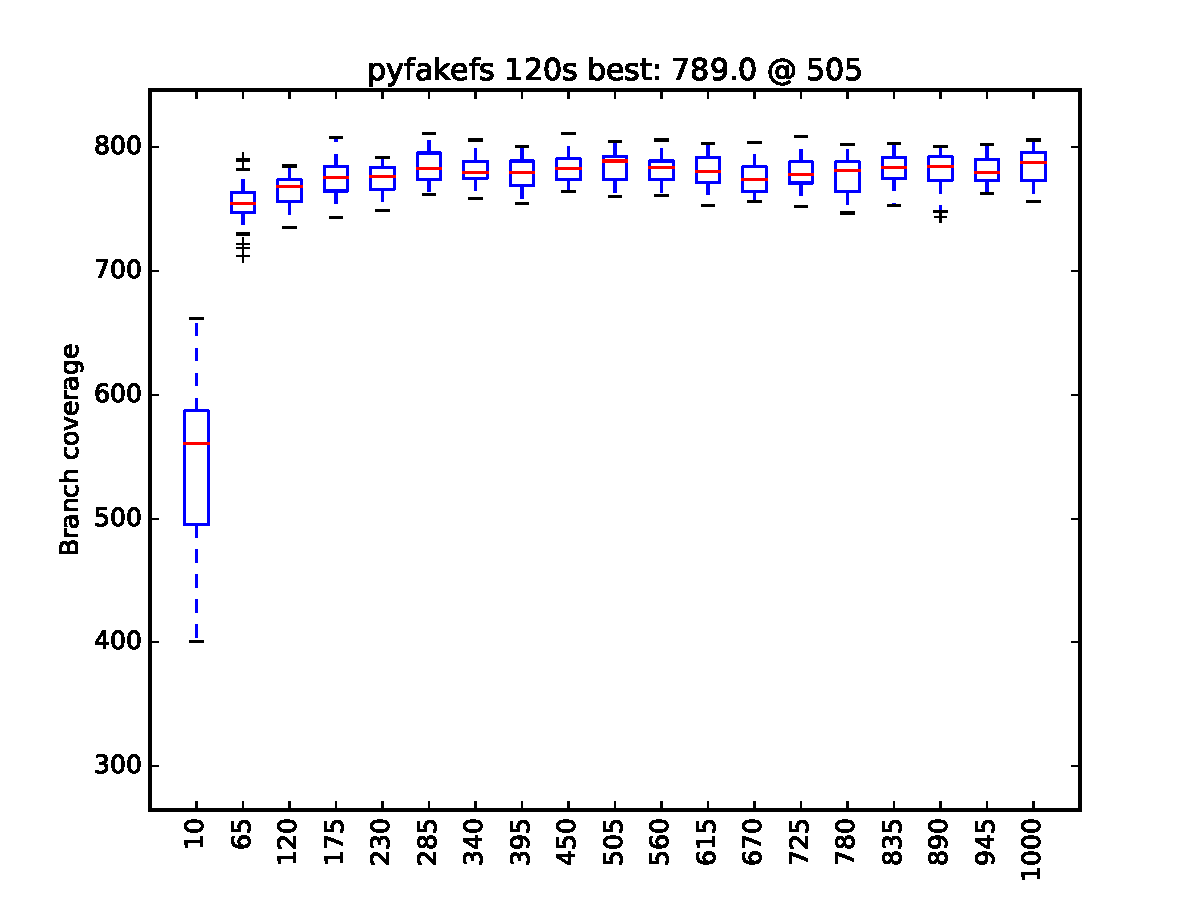
\includegraphics[width=0.9\columnwidth]{graphs/pyfakefsrand120}
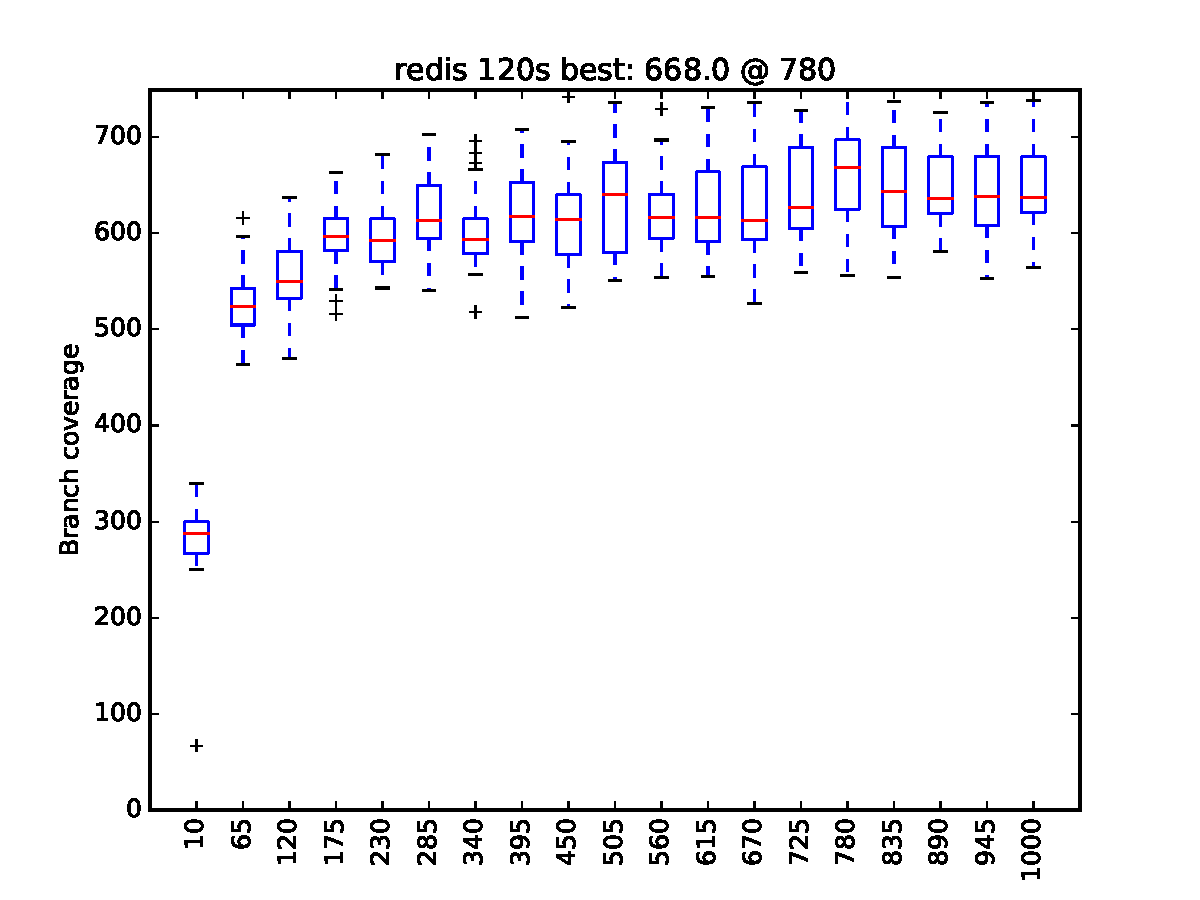
\includegraphics[width=0.9\columnwidth]{graphs/redisrand120}
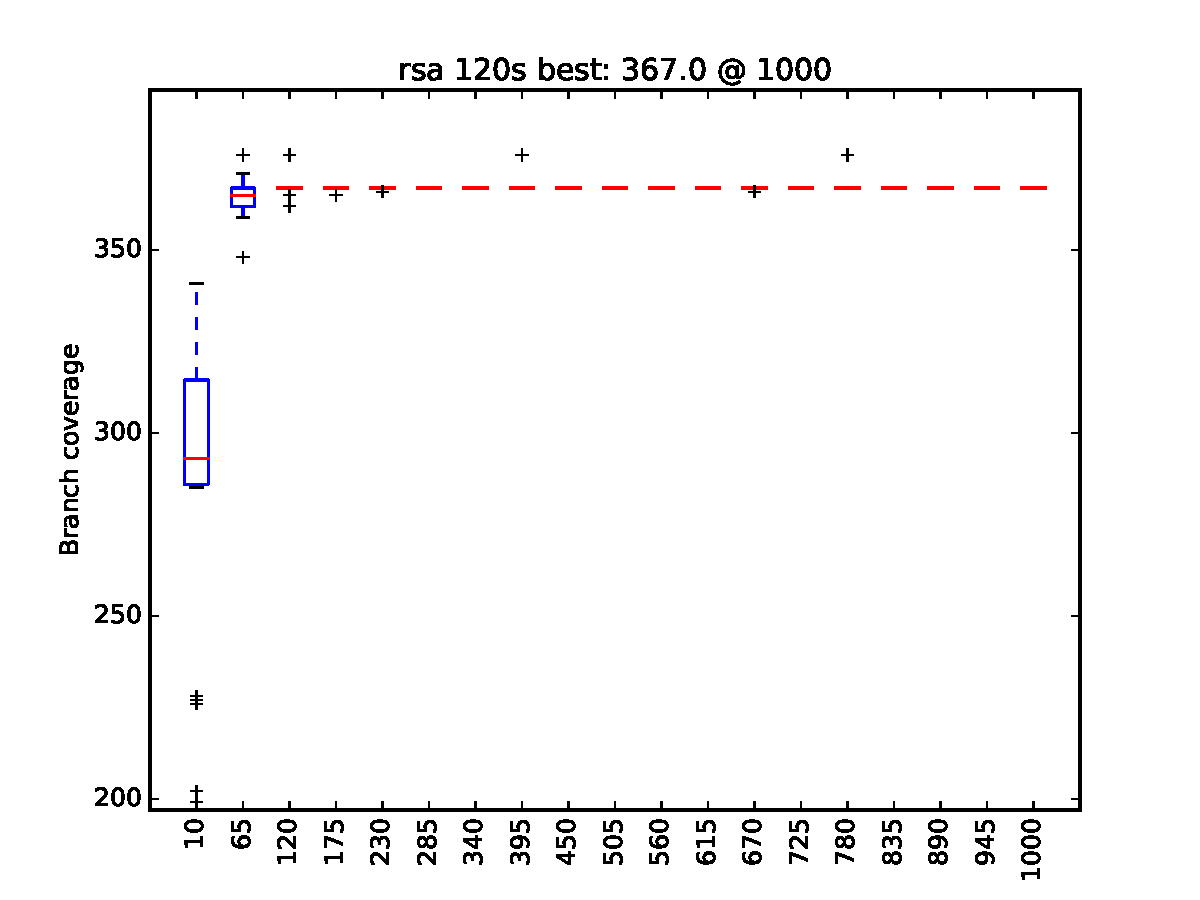
\includegraphics[width=0.9\columnwidth]{graphs/rsarand120}
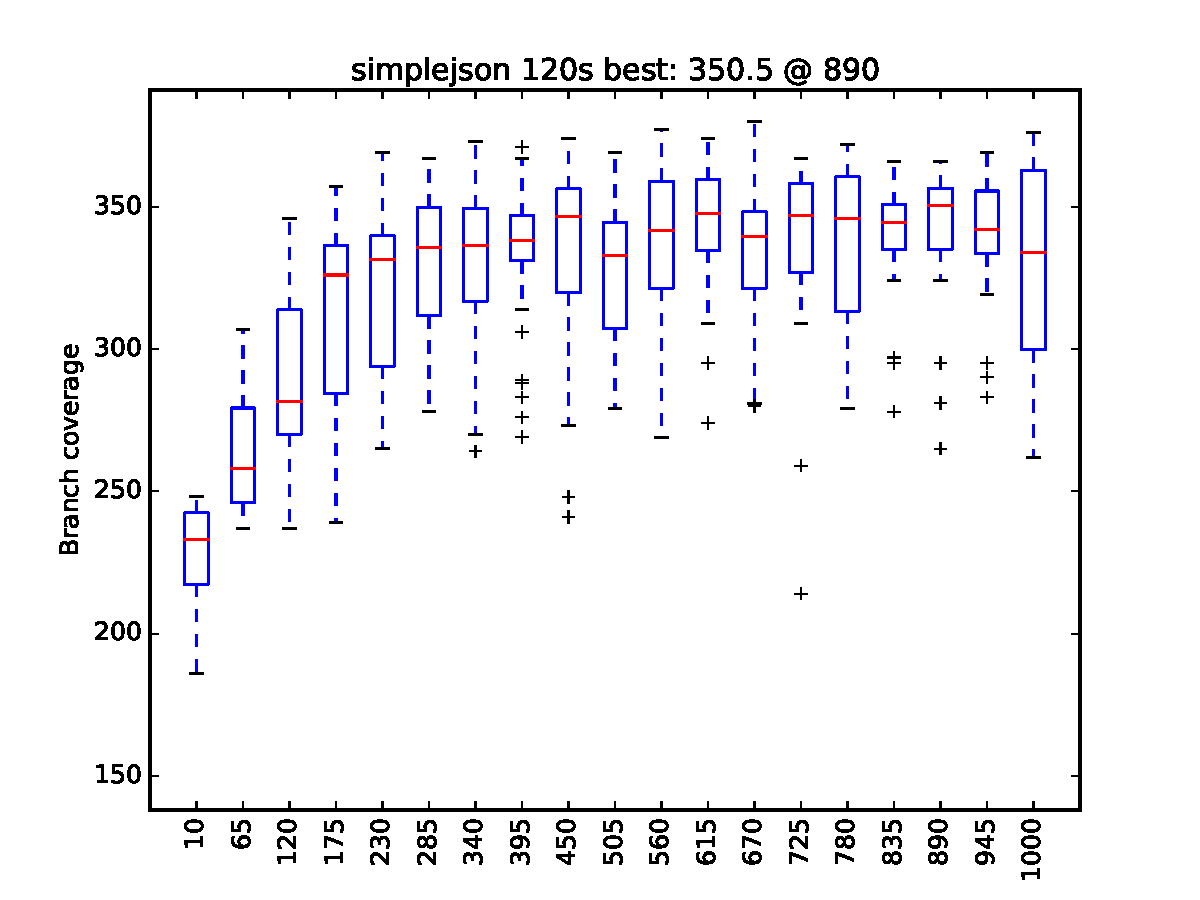
\includegraphics[width=0.9\columnwidth]{graphs/simplejsonrand120}
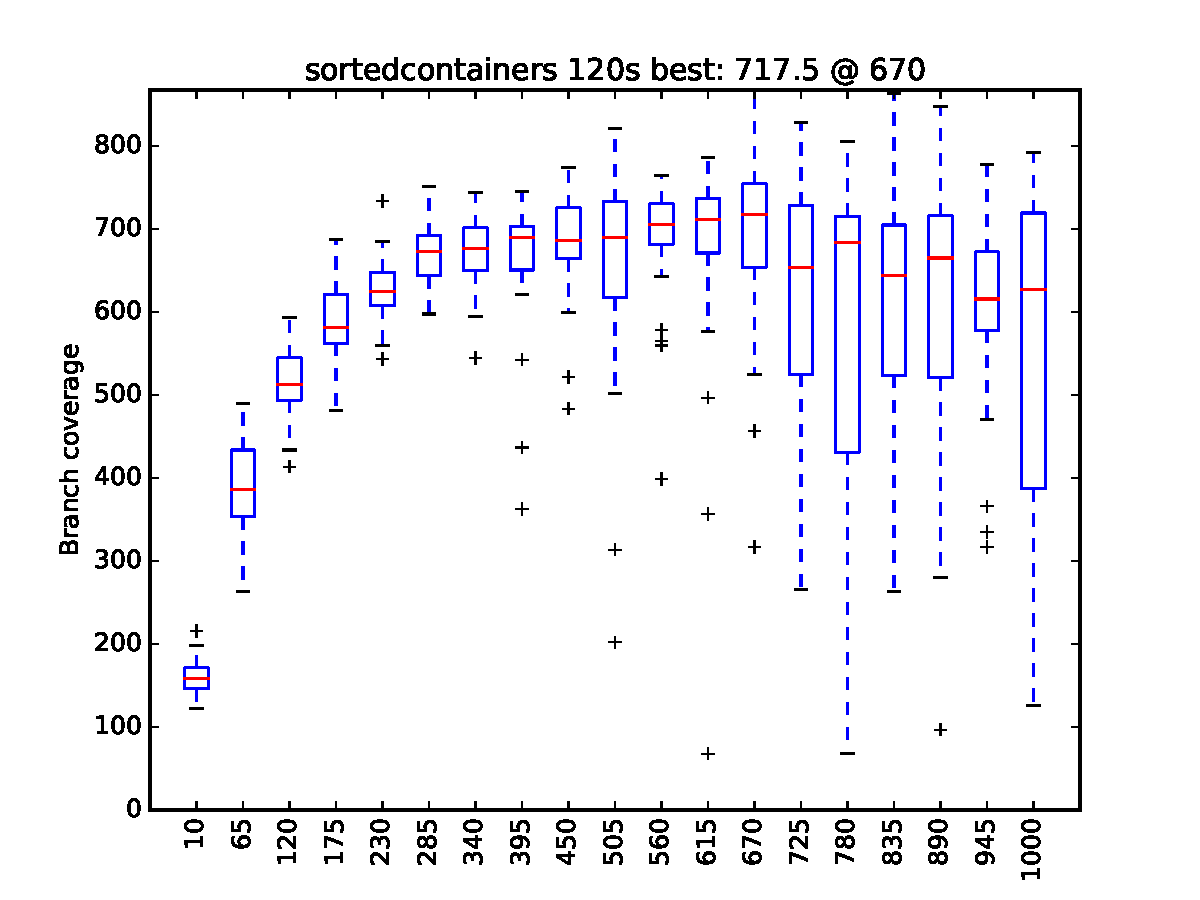
\includegraphics[width=0.9\columnwidth]{graphs/sortedcontainersrand120}
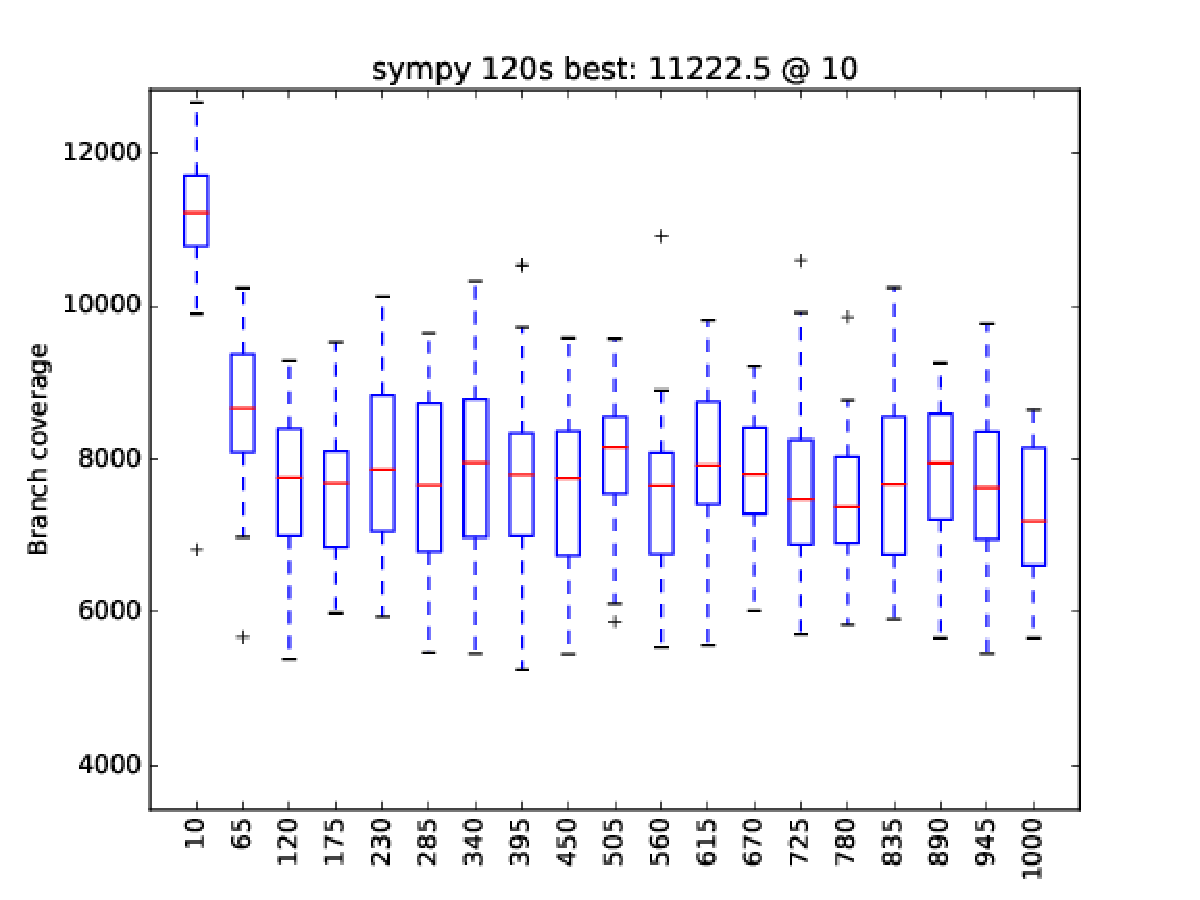
\includegraphics[width=0.9\columnwidth]{graphs/sympyrand120}
\caption{Best Test Lengths for Branch Coverage of Various Python
  Libraries}
\label{fig:length}

\end{figure*}

Figure \ref{fig:length} shows the range of branch coverage achieved in
two minute runs of the Python property-based API-sequence testing tool
TSTL \cite{tstlsttt}, for
eight real-world libraries.  The x-axis shows test sequence lengths,
and the y-axis branch coverage achieved over 100 repeated runs.  For
each method, the ``optimal'' test length is noted; this length ranges
from 10 to 1000 (the maximum length I used in experiments).  However,
just because the optimal length for a library is high or low does not
mean that some branches and bugs for that library don't need a very
different test length.  For every single target, at least two branches
were found where the optimal length for detecting \emph{that branch}
was not within 100 of the optimal value.  For {\tt pyfakefs}, {\tt
  sympy}, and {\tt sortedcontainers}, I know for a fact that real
bugs, which I reported, are most easily found using different test
length choices than the optimal value, and moreover, from each other.
In fact, for every program for which I have reported bugs, the bugs
``live'' at different test lengths.

It's not hard to understand why:  consider a bug that is caused by an
uninitialized value.  Imagine there are two function calls, {\tt foo}
and {\tt bar}.  If you call {\tt foo}, it will, as a side effect of
some other activity, initialize the uninitialized value.  In any given
test sequence, after there is a call to {\tt foo}, the bug will no
longer be detectable.  If you call {\tt bar}, but haven't first called
{\tt foo}, on the other hand, the bug will immediately be detected,
given certain choices for parameters to {\tt bar}.  In this case,
rather than running a smaller number of long tests, where any testing
after {\tt foo} is called cannot find the bug, it is best to run a
great number of fast, short, tests, in the hopes of hitting the right
{\tt bar} call before {\tt foo} shows up.

On the other hand, consider the classic overflow bug, where calling
{\tt baz} 64 times in a row causes no problems, but calling {\tt baz}
the 65th time overflows a fixed-size buffer and causes a crash.  If
there are 20 different calls that can be made, and the length of a
test is fixed at 100 calls, it's pretty hard to call {\tt baz} enough
times to trigger the bug before the ``deadline.''

As these examples show, the ``kinds of things'' that generated tests
do really vary depending on the length of tests.  In general, perhaps,
``longer is better'' \cite{ArcuriLen} but for any particular target
(bug or branch) you may be better off using diversity than optimality.

Thus, if you are using a test generation tool that lets you control
the length of inputs, and especially of call sequences, it is a very
good idea to vary the length parameter; it's a cheap way to get
significant diversity in your testing, almost like running different
tools without all the hassle!

\subsection{Swarm Techniques}

\begin{figure}
  \centering
  
\includegraphics[width=\columnwidth]{swarm.png}
  \caption{Kitchen-sink (top) vs. Swarm (bottom)}
  \label{fig:swarmcol}
\end{figure}

Figure \ref{fig:swarmcol} shows the basic logic of swarm testing
\cite{ISSTA12}.  The figure shows a 1,000x1,000 array of pixels, where
each 10x10 block represents a sequence of 100 function calls in
an API sequence test.  Each pixel is a call to a function, and the
calls to five different functions are coded by color (black, white,
red, green, and blue).  The top half of the figure is what traditional
sequence generation will tend to do in such a setting, assuming each
call is given equal probability:  every test will look like every
other test.  The details will vary, but at a certain level the
arrangement will be very homogeneous; in fact, the eye can't tell where
one test ends and another begins!  Let's call this the kitchen-sink
approach to testing:  every test generated throws in everything it can, at
least potentially.

The bottom half of the figure represents \emph{swarm testing}.  In
swarm testing, before each test is generated, a coin is flipped for
each of the five calls.  If the coin turns up ``heads'', then that
call is potentially included in the test; if the coin turns up
``tails'' the call is not made at all \emph{in this test}.  On
average, the diversity between calls within each test is \emph{much
  worse} for the swarm portion of the testing.  However, it is easy to
tell tests apart, with practical consequences.  Beyond the visually
obvious impact of swarm testing, there is simple statistical reality.
While it is \emph{possible} for a single method to be called 100 times
using the kitchen-sink approach, the most instances of any single call
we observed was 37.  For the swarm tests, of course, each method was
called more than 50 times (and in fact 100 times) in multiple tests.
The set of behaviors is simply larger, and more diverse.  You'll \emph{never}
see a pure-red, or red-green, kitchen-sink test, even if it's
technically possible.  Probability is more important than
possibility.  A million monkeys \emph{might} write Shakespeare, but
perhaps it's best not to throw away your Riverside edition, just yet.

More concretely, consider the problem of testing a stack
implementation that has incorrect overflow prevention code.  Imagine
the stack max size is 64 elements, and that the overflow allows
writing to the 65th element ({\tt stack[64]}), which will be detected by some form of
memory safety analysis.  If the stack has five methods we are testing,
{\tt push}, {\tt pop}, {\tt clear}, {\tt top}, and {\tt size}, and we
assign equal probability to calling each of these methods, then random
testing will tend to never generate a stack with 64 elements, that
could expose the bug on a push.  Rather, the mean stack size will be
quite close to zero, and the maximum size reached in a test of length
100 will also be quite small.  In swarm testing, on the other hand,
one in eight generated tests will omit {\tt pop} and {\tt clear} and
include {\tt push} and so tend towards a quite large stack size.  One
in 32 tests will omit all calls \emph{except} {\tt push}, guaranteeing
detection of the bug.  The case is exactly analogous to the figure: if
{\tt push} is represented by {\bf red} pixels, then the red ``dots''
in the bottom part of the figure represent tests guaranteed to detect
the bug.  In the top half of the figure, note that no square has a
dominant red shade, so no tests would expose the bug.

The statistical impact of swarm testing is relatively easy to measure
in a simple setting like this: the standard deviation of pixel counts
for each color in the swarm image is more than five times higher than
for the ``kitchen sink'' method.  Diversity here is easily measured as
increase in variance.

Swarm testing probably works because most coverage targets, and most
bugs, likely \emph{rely} on including some test features (e.g.,
function calls), which can be designated \emph{triggers}, but also are
\emph{prevented} by other function calls (designated
\emph{suppressors}).  In experiments, most targets and bugs in C
compilers and file systems, at least, had a small number of triggers
and a small number of suppressors, and were ``indifferent'' to other
test features \cite{groce2013help}.  This makes sense; it is hard to
design software humans can understand and use (much less implement
successfully) where every
functionality is intimately related to every other functionality\footnote{Dijkstra famously \cite{ewd} notes that the text of a
program should correspond to its execution structure if we are to have
any hope of working with it; the same factor limits most interfaces
(and perhaps can help focus testing)}.
Given this fact about the organization of software interfaces, it is
clear that diversity of ``kinds'' of tests, in terms of features
(elements of the interfaces) included is likely to be useful.

Swarm testing is fairly widely adopted in automated test generation.  It is frequently
applied to compiler testing \cite{le2014compiler,dewey2015fuzzing} and
is a core element of the testing approach used for FoundationDB, the
back-end database for Apple and Snowflake cloud services
\cite{zhou2021foundationdb}.  Tools implementing some form of swarm
testing include TSTL \cite{tstlsttt}, DeepState \cite{goodman2018deepstate}, and the very widely used Hypothesis
framework \cite{hypothesis}\footnote{See \url{https://github.com/HypothesisWorks/hypothesis/issues/2643}.}.
Via DeepState, swarm testing can be used in function call or
string generation in fuzzers such as afl and libFuzzer that do not
natively implement a notion of swarm testing.

Swarm testing was inspired by swarm verification \cite{swarmIEEE},
which makes explicit-state model checking more effective by applying a
variety of (often bad, but sometimes very good) tweaks to search
parameters, effectively using a variety of model checking algorithms.
Swarm verification is, arguably, essentially an \emph{ensemble method}.

\subsection{Ensemble Methods}

Finally, ensemble fuzzing \cite{chen2019enfuzz} is an approach that recognizes the need for
diverse methods for test generation, at least in the context of
fuzzing.   Inspired by ensemble methods in machine learning \cite{dietterich2002ensemble},
ensemble fuzzing runs multiple fuzzers, and uses inputs generated by
each fuzzer to seed the other fuzzers.  Ensemble fuzzing is currently
supported by the Enfuzz website  (\url{http://wingtecher.com/Enfuzz})
and by the DeepState front-end\footnote{See
\url{https://blog.trailofbits.com/2019/09/03/deepstate-now-supports-ensemble-fuzzing/}.}.

Less needs to be said about ensemble approaches than the other
examples of how to add diversity.  The whole point of ensemble methods
is that a tool takes care of the diversity for you.

\section{The Totalizing Nature of the Experimental Results Section}

\subsection{How it Is}

In software testing conference papers, whether on fuzzing or on other test
generation approaches (e.g., search-based testing \cite{McMinn04search-basedsoftware}), the basic
expectation is that there will be a research question like this:

\begin{quote}
\noindent {\bf RQ-N}:  Does {\bf our method} work better than {\bf competing
  methods} for testing basically all programs we tried?
\end{quote}

\noindent and an answer like

\begin{quote}
\noindent {\bf Our method} found a mean of 5.6\% more faults than all
other methods, including $N$ previously undiscovered faults.  {\bf Our
  method} also improved code coverage, covering 3.4\% more branches
per run on average.  Both results are statistically significant by
Mann-Whitney U test \cite{arcuri2014hitchhiker}, with $p < 0.001$.
\end{quote}

If the answer to {\bf RQ-N} is more nuanced than this, it is likely to result in
at least one reviewer (which may be fatal at better conferences) or
all reviewers questioning if the approach is really very useful, and
if it is worth spending the precious time and space of the conference
on such inconclusive results.

There are ways around this; one way is to hide the complexity of the
results via various subterfuges, or to restrict the set of of subject
programs to those whether the method worked, or just to lie; but we
will restrict our attention to \emph{honest} researchers.

It is permissible to write a paper with a subtler answer if you can
\emph{clearly define} the nature of the subtlety.  For example, if
your method is good for a particular kind of bug, then you can write a
paper with a title like ``A Method for Generating Tests to Detect {\bf
  CATEGORY} Bugs'' and then {\bf RQ-N} can be answered thus:


\begin{quote}
\noindent {\bf Our method} found a mean of 5.6\% more {\bf CATEGORY} faults than all
other methods, including $N$ previously undiscovered faults.  For
non-{\bf CATEGORY} faults, we found a mean of 8.1\% fewer faults than
other methods. {\bf Our
  method} decreased code coverage, covering 3.4\% fewer branches
per run on average.  However, when we identified branches associated
with {\bf CATEGORY} behavior, we improved code coverage by a mean of
1.4\%.  All results are statistically significant by
Mann-Whitney U test \cite{arcuri2014hitchhiker}, with $p < 0.001$.  We
conclude that our approach is successful at finding {\bf CATEGORY} bugs.
\end{quote}

However, either {\bf CATEGORY} must be a known, accepted, and
well-defined type of bug of general interest, or the bulk of the paper
must be spent explaining and defending the introduction of {\bf
  CATEGORY}.  The success of the paper in being published will depend
on whether reviewers decide that {\bf CATEGORY} cleaves nature at the
joints, or at minimum that {\bf CATEGORY} relates to some hot topic of
the day.

The basic expectation is \emph{totalizing}.  A good research paper in
software testing will define a problem (perhaps a specialized, {\bf
  CATEGORY}-defined problem), and then present a \emph{new, best} way
to solve that problem.

\subsection{How it Should Be: Taking Diversity Seriously}

Accepting any test generation paper where a method found at least one
new bug would flood the research literature with uninteresting
results.  The situation described above did not arise through malice
or ignorance, but through the desire of program committee members to
weed out bad work.  Nobody wants to fill ICSE or ISSTA with papers
that end with a whimper, not a bang, e.g.:

\begin{quote}
\noindent {\bf Our method} found a mean of 2.6\% fewer faults than all
other methods.  {\bf Our
  method} also decreased code coverage, covering 1.4\% fewer branches
per run on average.  Both results are statistically significant by
Mann-Whitney U test \cite{arcuri2014hitchhiker}, with $p < 0.001$.
\end{quote}

Cowper, introducing his notion that variety is the spice of life,
concluded that variety isn't all it is cracked up to be, and often
leads simply to ``monstrous novelty and strange disguise.''  In
practice, however, this is not a realistic danger.  Program committees
will not accept many papers that end in a simple ``our method did not
work.''  However, it is also true that program committees, in a
not-so-distant past, did probably accept too many interesting ideas
evaluated poorly on toy problems\footnote{In part, the current problem is a
result of the increasing maturity of the field; learning how to evaluate research
is often a challenge for emerging fields \cite{10.1145/1294211.1294256}.}.

There is a place for negative results, but most papers published
should probably introduce \emph{useful} methods.  However, what if the
answer was something like this?

\begin{quote}
\noindent {\bf Our method} found a mean of 2.6\% fewer faults than all
other methods.  {\bf Our
  method} also decreased code coverage, covering 1.4\% fewer branches
per run on average.  Both results are statistically significant by
Mann-Whitney U test \cite{arcuri2014hitchhiker}, with $p < 0.001$.
However, for 75\% of subject programs, for at least $k$ faults and $b$
branch coverage targets, our approach improved the probability of
detection per test by a factor of $10$ or more, compared to all other
methods.  There was no way to predict which faults or branches would
be thus affected.  We speculate that the underlying combinatorics of
inputs relate to our use of {\bf new technique}.
\end{quote}

Assuming that standards are set high enough for $k$ and $b$, and
perhaps with some expectation that published methods at top
conferences will show discovery of at least one novel fault, this
seems like a potentially very useful result.  In particular, the
baseline comparison in a well-written paper is likely to be the set of
widely-used methods at present.  A problem facing most serious testing
(especially fuzzing) efforts is that of saturation:  you keep fuzzing
with good tools, and you don't find any new bugs, or even add any new
interesting inputs to your corpus, except when major changes are made
to the code under test.  Are you done?  Is the fuzzing ``finished''?
Probably not, unless the program under test is fairly trivial.  The
problem is serious, and common.  I myself was contacted by the team
testing the bitcoin core implementation, after publishing (with John
Regehr) a blog post
on saturation\footnote{See
  \url{https://blog.regehr.org/archives/1796}.}.

One way to get out of saturation is to apply ``worse'' but useful
methods.  You used the best fuzzer, and the second-best fuzzer.  Now
try the fourth best fuzzer, and a brute-force really dumb but fast
fuzzer, and this ``one weird trick'' that sometimes works, the
literature shows.  In the absence of a more diversity-aware
literature, this kind of thing has to be done, but there's not a good,
principled, peer-reviewed set of guidelines on how it should be done.
For bitcoin core, the work is in progress, but simply running more
fuzzers than the best-performing one (libFuzzer, in this case), for
longer periods proved helpful.

Our research field is, to a large extent, failing to curate the
literature on specialized, but ill-defined, test generation methods.
The criticality of diversity, and in particular the problem of
saturation, however, means that such specialized methods are likely
\emph{needed} in any truly high-stakes testing effort.

There is no denying that this places more burden on the program
committee.  The standards for what is a good-enough paper are already
hard to realize; accepting the best partial methods means that in
addition to scrutinizing experiments, reviewers have to give a lot
more thought to the question of whether the underlying approach
described makes sense, is unusual and not just an incremental
improvement to a known method, whether it is well-enough described to
make it plausible the partial results aren't just luck, and so forth.
However, as it is, the approach tends to make it hard or impossible to
publish many useful methods in many software engineering and testing
conferences.  It is likely that junior researchers, under the pressure
to publish or perish, may abandon research on methods that are fruitful, but
clearly specialized and unable to honestly climb over the hurdle of
the expected {\bf RQ-N} answer.

Software testing is \emph{hard}.  We need every genuinely useful, even
specialized, tool we can discover, in order to find bugs.  Right now,
we're forcing test generation methods, in order to obtain publicity,
to satisfy unrealistic constraints, and thereby rejecting many tools
that probably should be in our belts.

\subsection{How to Get Around It}

In the absence of more diversity-friendly reviewers, there are ways to
publish work on promising partial testing approaches.  Each of these
approaches has at least one major problem, however, in practice.

\subsubsection{Journal Papers}

Conference program committees basically only have the option to reject
a paper with a weak answer to {\bf RQ-N} or an unconvincing {\bf
  CATEGORY} concept.  In fact, the original swarm testing paper was
rejected once, due to a single annoyed reviewer who said ``this only seems useful for
testing systems software'' (with the implication, presumably, being
that nobody would want to do \emph{that}).  Journal papers are a more
collaborative kind of publication; unless the idea is just
uninteresting or the results are \emph{terrible}, it's possible to go
back and forth and present a nuanced set of results.  For one thing,
there's space to elaborate on how often a method works, and explain
that it is sometimes useful and sometimes not useful.  A recent paper
in TOSEM, where I had the honor of working the idea of a brilliant
student through the process, after the student left the field,
exemplifies the result \cite{HolmesLOC}.  The paper had trouble at
conferences because the results showed that sometimes the proposed
test generation heuristic was harmful, and for some programs resulted
in much worse results.  At conferences, even with a modest overall
improvement (a middling-good {\bf RQ-N} answer), that was fatal.  In
the expansive world of a journal paper, even at a top journal, it was
acceptable to describe the highly varying results (sometimes the
method was very powerful, and sometimes seriously detrimental), and
even spend some time extolling diversity of methods.  The journal
setting gave us room to even spend some time expanding on the virtues
of competing approaches.  This is probably, right now, the best way to
publish the best partial methods.

The problem is that people don't seem to read journal papers as much
as they read conference papers.  In practice, unless you have a wide
following that reads all of your papers, even a TSE or TOSEM paper
isn't going to obtain the audience that an ICSE or even ISSTA paper
will.  I tend to go look at the titles of the accepted papers lists for the
top conferences in the field, to see if anything sounds exciting, but I only see a good TSE or TOSEM
paper when Google Scholar decides to send me an alert.

Also, the turnaround for journal papers remains slow, so this
may or may not be a useful avenue for junior researchers, depending on
how they are evaluated.  Finally, journal papers in good journals generally expect a
very high standard of evaluation, much more than a conference paper
will typically require for a promising and interesting-sounding
method.  The iterative process where reviewers collaborate with
authors, that makes it possible to publish partial results, also means
that a published paper will likely incorporate various new experiments
or evaluation measures demanded by reviewers as the price for
admission.  This is sometimes good, for readers of the paper, but can make the required effort,
for junior faculty, or graduate students wanting to finish their PhD,
look bad in a cost-benefit analysis.  More importantly, it can delay
the publication of important new methods that might be extremely
useful in escaping saturation or as an addition to ensemble methods.

\subsubsection{Ensemble Evaluation}

Speaking of ensemble methods, one interesting way to get around the totalitarian results section
expectation is to ``cheat'' by adding your method to an ensemble
approach.  If you can show that, e.g., Enfuzz + {\bf New Method} does much
better by the traditional {\bf RQ-N} standards, that may be enough to
satisfy non-diversity-tolerant reviewers.

The problem is that ensemble frameworks are either fairly new and
unstable (in fuzzing) or, to our knowledge, non-existent in many other
automated test generation settings.  This route may require
substantial engineering effort, and some part of the paper will have
to be devoted to justifying the use of an ensemble evaluation.

\subsubsection{Preregistration}

One interesting way around the {\bf RQ-N} wall is the use of
preregistration.  In preregistration, authors propose a method, and
a paper is accepted or rejected based on how interesting and likely to
be useful the method sounds.  Only \emph{after} in-principle
acceptance or rejection is an evaluation conducted.  Thus, if the
method sounds good, and the {\bf RQ-N} result is nuanced, the paper is
still accepted.  Proponents of preregistration argue that the approach
avoid duplicated efforts, by allowing for the publication of negative
results, and reduces the temptation for authors to over-claim in
results sections.  A group of top testing researchers has proposed to
use preregistration to address problems in ``the incentive structure
for fuzzing research'' and is planning to organize a journal issue to
address the problem \cite{special}.  In practice, preregistration as a solution to
publishing partial solutions is a subset of the journal solution,
because by and large, well-known conferences in the field do not currently allow
for preregistration.


\subsubsection{Build a Tool}

Finally, if your testing work is not driven by the academic (or
industrial lab) publish-or-perish imperative, you can find an
interesting method and either build a tool that implements it, or add
it to an existing tool.  Testing tools and fuzzers are now widely used
enough that if your approach is useful enough, even if only for some
bugs, it may find an audience.

The problem is that this doesn't work for everyone, due to career
needs \footnote{This essay may convince PCs that diversity is good,
  but it will never convince most promotion and tenure committees at
  universities that a tool that doesn't make the front page of the New
  York Times is worth even one minor journal publication.}.  Also, in practice,
unless you have a base in a famous company or university, there are a
lot of tools out there and nobody is going to hear about your tool.
There are exceptions, such as David R. MacIver's Hypothesis, but by
and large it is at least as hard to get attention for even a very
useful new tool, unless you have an existing audience for your work,
as it is to get attention for a new research paper or result.  It is
possible that using a tool to find bugs in important software is a way
around this, but this requires a lot of work for uncertain payoff.

\section{Conclusions}

Software testing is a kind of scavenger hunt for the set of all bugs,
where the consequence of not finding even one item on the (invisible)
list may be a major security breach, the loss of a Mars mission, or
the loss of human life.  In practice, there are no silver bullets, no
testing methods that are best for all bugs, and so the use of a
variety of approaches is essential in serious testing efforts.  There
are existing practical ways for those who really want to find all the
bugs to take advantage of diversity.  However, it is likely that the
available tools and methods are less diverse than they could be and
should be, because of certain expectations of the research community.
While these expectations are based on a desire to ensure the quality
of testing research, they exclude important results.   This essay
offers no simple solution to this problem, but proposes that the
software testing research community should begin to explore how to
accept the reality that even some ``poorly performing'' testing methods may
be essential foot soldiers in our war on error.

{\bf Acknowledgments:} The author would like to thank the 
reviewers, and would particularly like to thank Tomas Petricek for a
very interesting, \emph{signed} review; the limits of time and my own
understanding prevented me from making use of all his suggestions, but
I now have {\bf Image and Logic} on my reading queue, among other
things.  I would also like to thank numerous colleagues and
collaborators for their discussion of these topics over many years; in
particular John Regehr, Josie Holmes, Gerard Holzmann, Peter Goodman,
Willem Visser, Mike Ernst, Andreas Zeller, and
Gustavo Grieco, as well as my graduate students and many students in my
software testing classes, have helped shape my thinking on these matters.

\bibliographystyle{plain}
\bibliography{bibliography}



\end{document}
